\begin{abcliste}
\abc With $d$ the distance of neighbouring ions, \ce{Na+} and \ce{Cl-} attract each other with
\begin{align}
 F_1 &= \FaF \\
   &= \kC\times\frac{\left(\qe\right)^2}{\left(\dn\right)^2} \\
   &= \Fa \approx \result{\FaP{-9}{2}}
\end{align}

\abc
\begin{center}
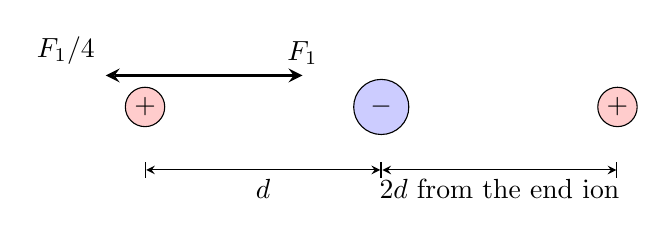
\begin{tikzpicture}[>=stealth]
 \draw[fill=red!20] (0,0) circle (0.25) node {$+$};
 \draw[fill=blue!20] (3,0) circle (0.35) node {$-$};
 \draw[fill=red!20] (6,0) circle (0.25) node {$+$};
 \draw[|<->|] (0,-0.8) -- node[below] {$d$} (3,-0.8);
 \draw[|<->|] (3,-0.8) -- node[below] {$2d$ from the end ion} (6,-0.8);
 \draw[->, very thick] (0,0.4) -- (2,0.4) node[above] {$F_1$};
 \draw[->, very thick] (0,0.4) -- (-0.5,0.4) node[above left] {$F_1/4$};
\end{tikzpicture}
\end{center}
The \ce{Cl-} ion pulls the end ion into the row with $F_1$; the \ce{Na+} ion at the distance $2d$ pushes it out with $F_1/2^2 = F_1/4$. The two forces lie on one line and point in opposite directions:
\begin{align}
 F &= F_1 - \frac{F_1}{4} = \FF \\
   &= \frac{3}{4}\times\Fa \\
   &= \F \approx \result{\FP{-9}{2}}
\end{align}
It points \emph{into the crystal}: the crystal holds its ions together.
\end{abcliste}
